\documentclass[11pt,a4paper]{article}
\usepackage[utf8]{inputenc}
\usepackage[french]{babel}
\usepackage[T1]{fontenc}

\usepackage{amsmath}
\usepackage{amsfonts}
\usepackage{amssymb}

\newcommand{\NomAuteur}{Fabrice BOISSIER}
\newcommand{\TitreMatiere}{Algorithmique 1}
\newcommand{\NomUniv}{EPITA - Bachelor Cyber Sécurité}
\newcommand{\NiveauUniv}{CYBER1}
\newcommand{\NumGroupe}{CYBER1}
\newcommand{\AnneeUniv}{2023-2024}
\newcommand{\DateExam}{décembre 2023}
\newcommand{\TypeExam}{CORRECTION Partiel}
\newcommand{\TitreExam}{\TitreMatiere}
\newcommand{\DureeExam}{2h00}
\newcommand{\MyWaterMark}{\AnneeUniv} % Watermark de protection

% Ajout de mes classes & definitions
\usepackage{MetalExam} % Appelle un .sty

% "Tableau" et pas "Table"
\addto\captionsfrench{\def\tablename{Tableau}}

%%%%%%%%%%%%%%%%%%%%%%%
%Header
%%%%%%%%%%%%%%%%%%%%%%%
\lhead{\TypeExam}							%Gauche Haut
\chead{\NomUniv}							%Centre Haut
\rhead{\NumGroupe}							%Droite Haut
\lfoot{\DateExam}							%Gauche Bas
\cfoot{\thepage{} / \pageref*{LastPage}}	%Centre Bas
\rfoot{\texttt{\TitreMatiere}}				%Droite Bas

%%%%%

\usepackage{tabularx}

\newlength{\LabelWidth}%
%\setlength{\LabelWidth}{1.3in}%
\setlength{\LabelWidth}{1cm}%
%\settowidth{\LabelWidth}{Employee E-mail:}%  Specify the widest text here.

% Optional first parameter here specifies the alignment of
% the text within the \makebox.  Default is [l] for left
% alignment. Other options are [r] and [c] for right and center
\newcommand*{\AdjustSize}[2][l]{\makebox[\LabelWidth][#1]{#2}}%


\definecolor{mGreen}{rgb}{0,0.6,0}
\definecolor{mGray}{rgb}{0.5,0.5,0.5}
\definecolor{mPurple}{rgb}{0.58,0,0.82}
\definecolor{backgroundColour}{rgb}{0.95,0.95,0.92}

\lstdefinestyle{CStyle}{
    backgroundcolor=\color{backgroundColour},
    commentstyle=\color{mGreen},
    keywordstyle=\color{magenta},
    numberstyle=\tiny\color{mGray},
    stringstyle=\color{mPurple},
    basicstyle=\footnotesize,
    breakatwhitespace=false,
    breaklines=true,
    captionpos=b,
    keepspaces=true,
    numbers=left,
    numbersep=5pt,
    showspaces=false,
    showstringspaces=false,
    showtabs=false,
    tabsize=2,
    language=C
}


\hyphenation{op-tical net-works SIGKILL}


\begin{document}

%\MakeExamTitleDuree     % Pour afficher la duree
\MakeExamTitle                   % Ne pas afficher la duree

%% \MakeStudentName    %% A reutiliser sur chaque nouvelle page

\bigskip
%\bigskip

Vous devez respecter les consignes suivantes, sous peine de 0 :

\begin{itemize}
\item Lisez le sujet en entier avec attention
\item Répondez sur le sujet
\item Ne détachez pas les agrafes du sujet
\item \'Ecrivez lisiblement vos réponses (si nécessaire en majuscules)
%\item Vous devez écrire dans le langage algorithmique ou en C (donc pas de Python ou autre)
\item Ne trichez pas
\end{itemize}

\bigskip

%%%%%%%%%%%%%%%%% CENTRAGE
\vfillFirst

% Questions cours
\section{Questions (6 points)}

\bigskip

\subsection{(2 points) En admettant que l'on dispose d'une pile et que l'on insère les données \og 1 2 3 4 5 6 \fg{} dans cet ordre exclusivement, décrivez les scénarios permettant d'obtenir les sorties suivantes : }
%%% PREFERER CE TEXTE :
%\subsection{(3 points) En admettant que l'on dispose d'une pile vide et que les éléments \og 1 2 3 4 5 6 \fg{} arrivent en entrée dans cet ordre exclusivement, décrivez les scénarios permettant d'obtenir les sorties suivantes : }

\bigskip

\begin{center}
\noindent \textit{exemple : pour \og A B C \fg{} en entrée, on peut obtenir \og B C A \fg{} en sortie en faisant : \linebreak
\og push A \fg, \og push B \fg, \og pop \fg, \og push C \fg, \og pop \fg, \og pop \fg }
%%% AJOUTER CE TEXTE :
%On a bien inséré A, puis B, puis C, mais l'ordre de sortie est différent suivant les \og pop \fg}
\end{center}

\medskip


\begin{center}

\begin{large}
3, 2, 4, 1, 6, 5
\end{large}

\begin{center}
%\GrilleReponseN{5}
push 1, push 2, push 3, pop, pop, push 4, pop, pop, push 5, push 6, pop, pop
\end{center}


\begin{large}
3, 5, 4, 6, 2, 1
\end{large}

\begin{center}
%\GrilleReponseN{5}
push 1, push 2, push 3, pop, push 4, push 5, pop, pop, push 6, pop, pop, pop
\end{center}

\end{center}

\vfillLast
%%%%%%%%%%%%%%%%% CENTRAGE

\newpage

\subsection{(2 points) Indiquez l'état de la liste après chacune de ces opérations, puis précisez à quelle structure de données ce comportement correspond. }

%\bigskip

\begin{figure}[ht!]
\centering
\centerline{  %%% CENTRAGE HORIZONTAL
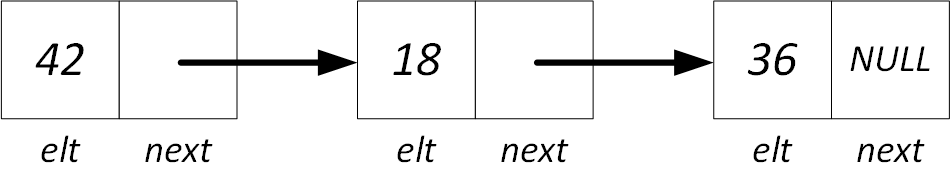
\includegraphics[height=1.85cm]{img/Liste_p_1.png}
%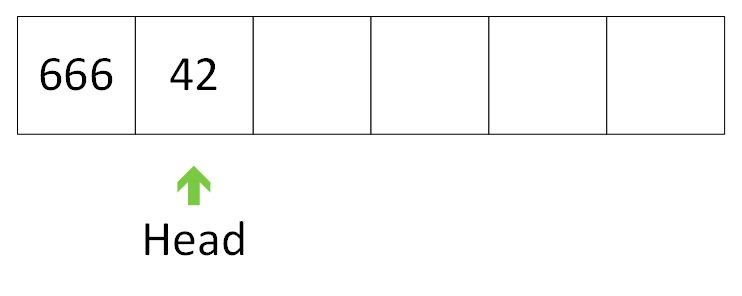
\includegraphics[scale=1,left]{img/2_elts.png}
}
\end{figure}

\begin{center}

%\begin{table}[h!]
%  \centering
%  \begin{minipage}{0.45\textwidth}
%    \centering
%\texttt{Ajout de 55 en première position}
%  \end{minipage}
%  \hfillx
%  \begin{minipage}{0.3\textwidth}
%  \end{minipage}
%\end{table}

\texttt{Ajout de 55 en première position}

\begin{figure}[ht!]
\centering
\centerline{  %%% CENTRAGE HORIZONTAL
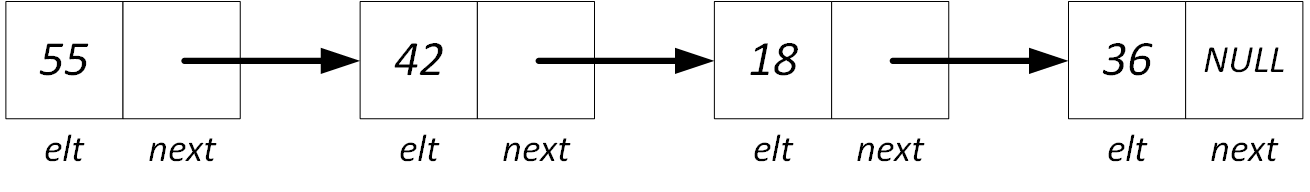
\includegraphics[height=1.85cm]{img/p-1-Liste_p_4.png}
%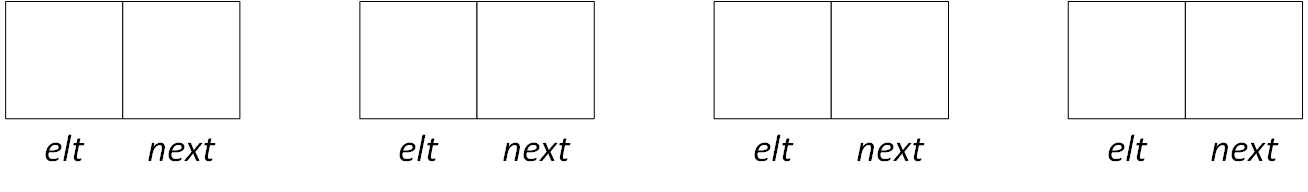
\includegraphics[height=1.85cm]{img/Liste_p_vide_4.png}
%%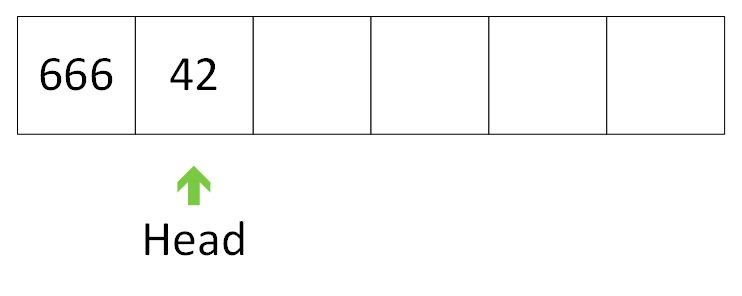
\includegraphics[scale=1,left]{img/2_elts.png}
}
\end{figure}


\texttt{Ajout de 14 en première position}

\begin{figure}[ht!]
\centering
\centerline{  %%% CENTRAGE HORIZONTAL
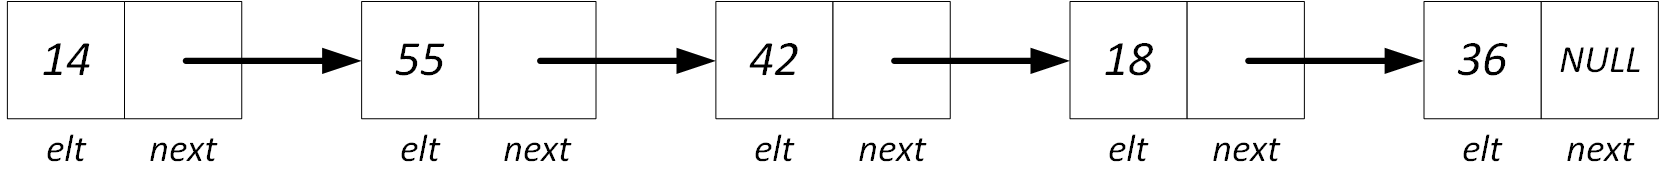
\includegraphics[height=1.85cm]{img/p-2-Liste_p_5.png}
%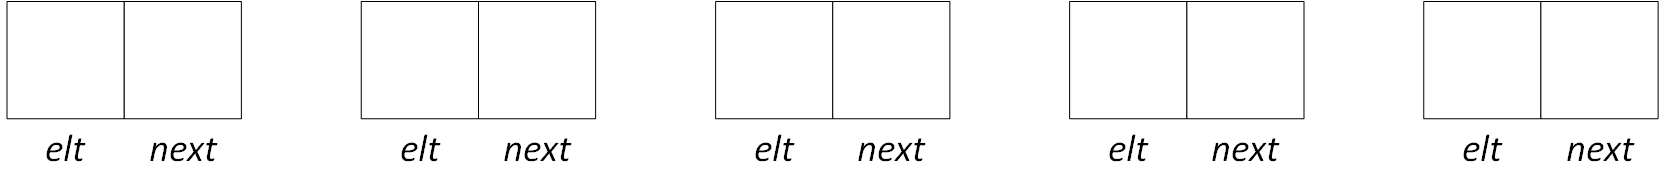
\includegraphics[height=1.85cm]{img/Liste_p_vide_5.png}
%%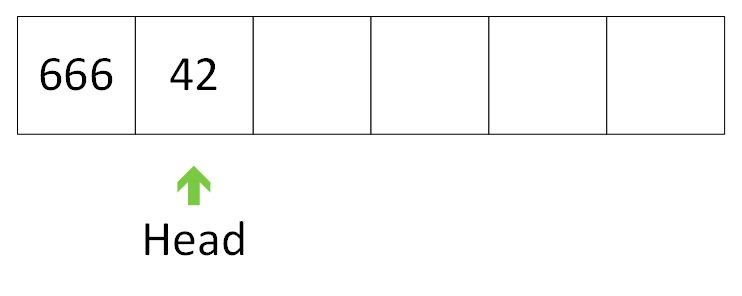
\includegraphics[scale=1,left]{img/2_elts.png}
}
\end{figure}


\texttt{Ajout de 21 en première position}

\begin{figure}[ht!]
\centering
\centerline{  %%% CENTRAGE HORIZONTAL
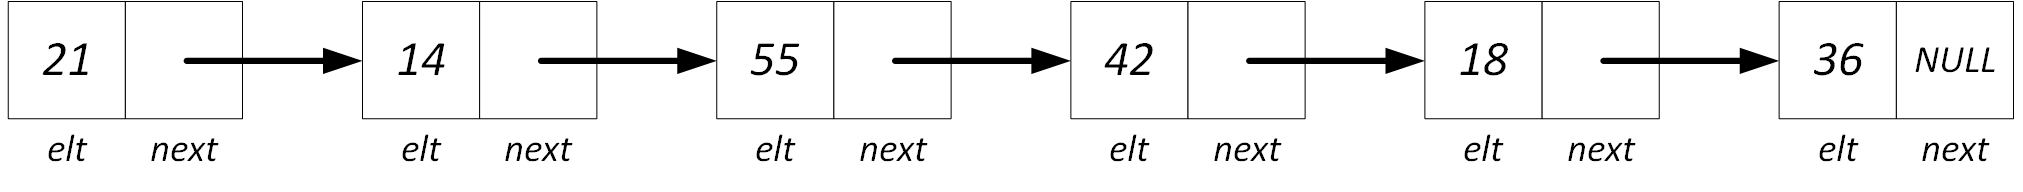
\includegraphics[height=1.85cm]{img/p-3-Liste_p_6.png}
%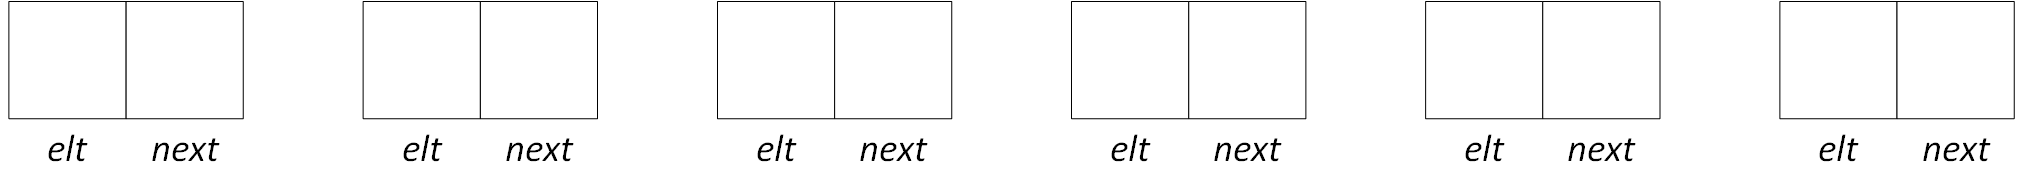
\includegraphics[height=1.85cm]{img/Liste_p_vide_6.png}
%%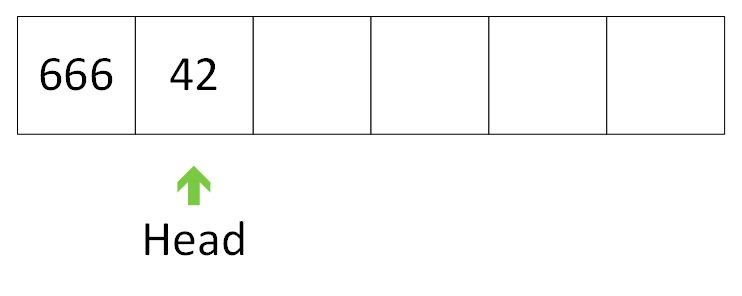
\includegraphics[scale=1,left]{img/2_elts.png}
}
\end{figure}


\texttt{Suppression de la première position}

\begin{figure}[ht!]
\centering
\centerline{  %%% CENTRAGE HORIZONTAL
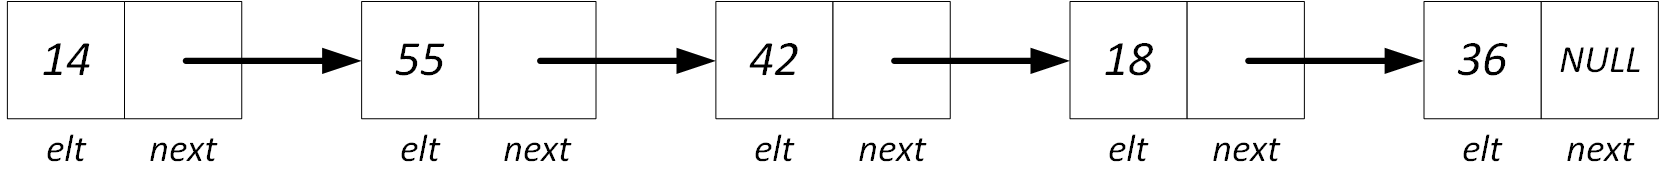
\includegraphics[height=1.85cm]{img/p-2-Liste_p_5.png}
%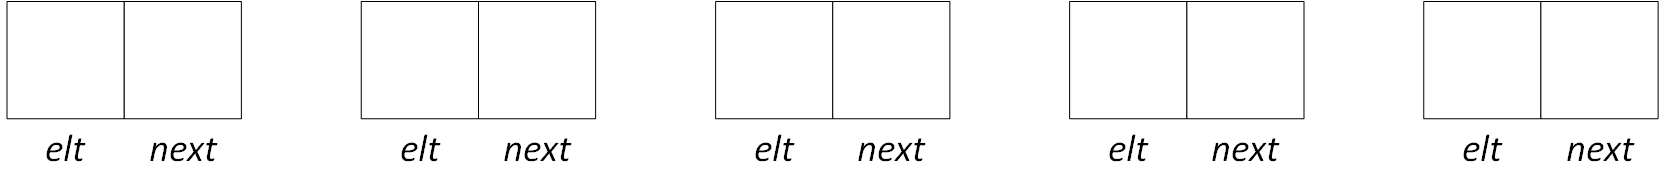
\includegraphics[height=1.85cm]{img/Liste_p_vide_5.png}
%%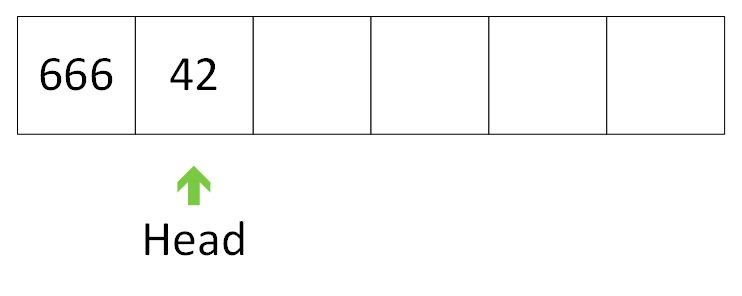
\includegraphics[scale=1,left]{img/2_elts.png}
}
\end{figure}


\texttt{Suppression de la première position}

\begin{figure}[ht!]
\centering
\centerline{  %%% CENTRAGE HORIZONTAL
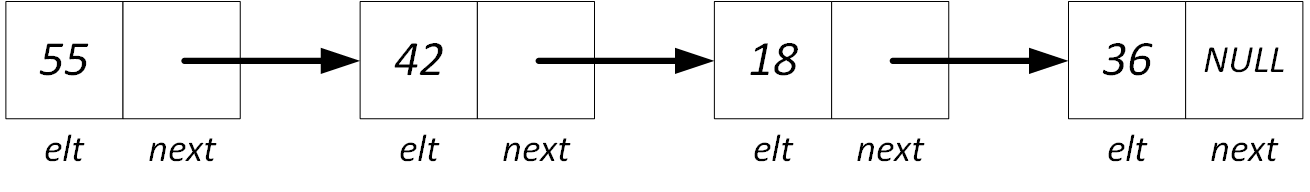
\includegraphics[height=1.85cm]{img/p-1-Liste_p_4.png}
%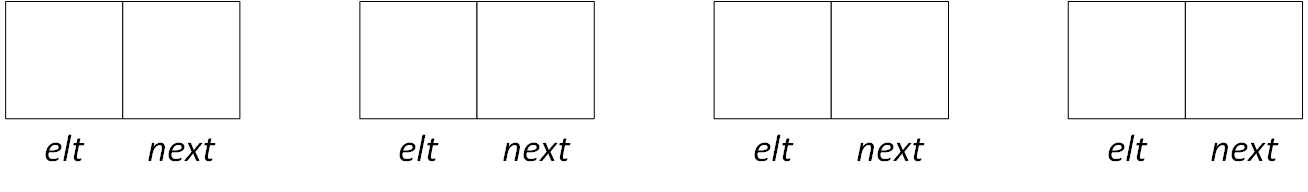
\includegraphics[height=1.85cm]{img/Liste_p_vide_4.png}
%%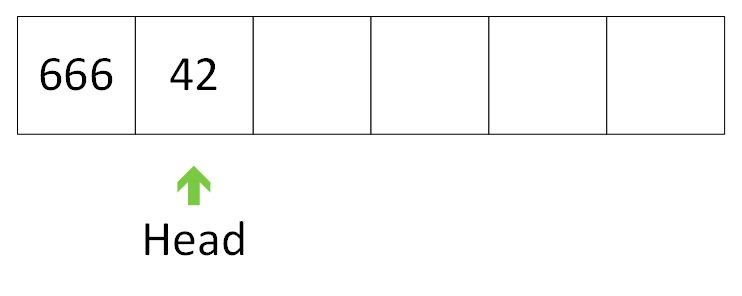
\includegraphics[scale=1,left]{img/2_elts.png}
}
\end{figure}


\texttt{Suppression de la première position}

\begin{figure}[ht!]
\centering
\centerline{  %%% CENTRAGE HORIZONTAL
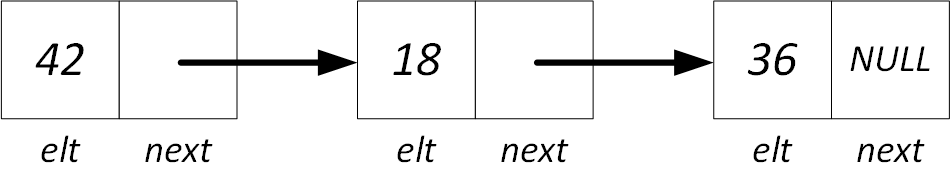
\includegraphics[height=1.85cm]{img/Liste_p_1.png}
%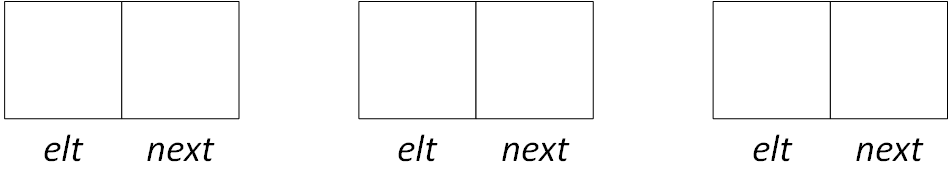
\includegraphics[height=1.85cm]{img/Liste_p_vide_3.png}
%%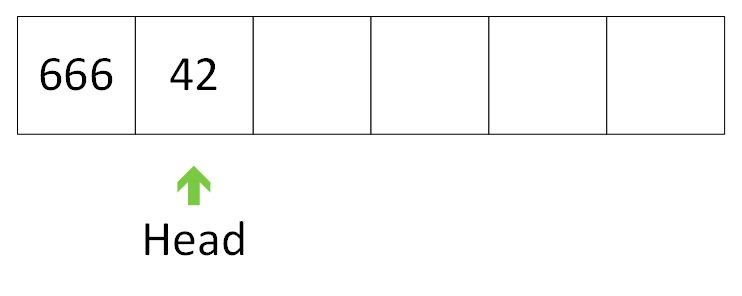
\includegraphics[scale=1,left]{img/2_elts.png}
}
\end{figure}

\bigskip

\end{center}

Structure de données imitée : \textbf{Pile}



\clearpage

\subsection{(2 points) Indiquez l'état de la liste après chacune de ces opérations, puis précisez à quelle structure de données ce comportement correspond. }

%\bigskip

\begin{figure}[ht!]
\centering
\centerline{  %%% CENTRAGE HORIZONTAL
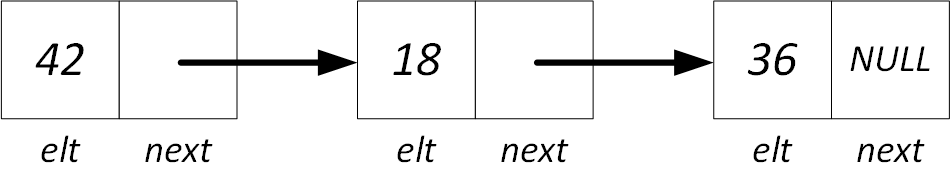
\includegraphics[height=1.85cm]{img/Liste_p_1.png}
%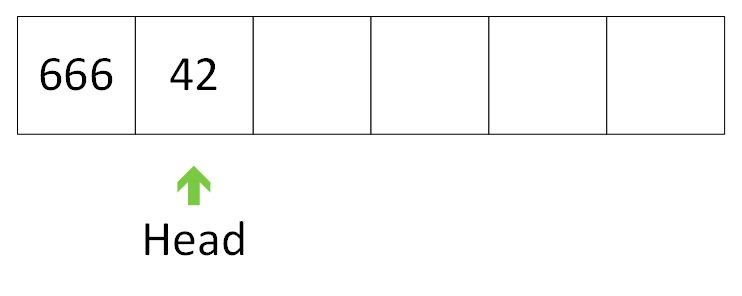
\includegraphics[scale=1,left]{img/2_elts.png}
}
\end{figure}

\begin{center}

\texttt{Ajout de 55 en \textit{dernière} position}

\begin{figure}[ht!]
\centering
\centerline{  %%% CENTRAGE HORIZONTAL
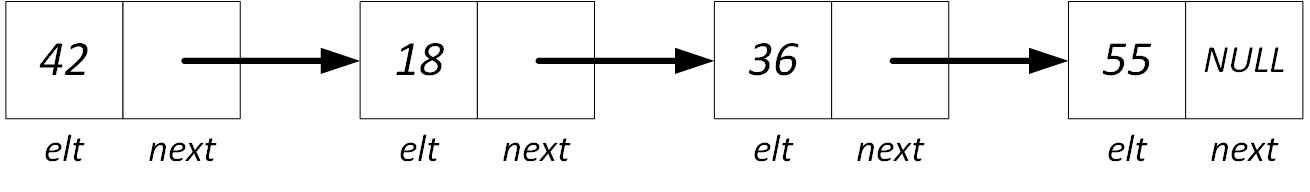
\includegraphics[height=1.85cm]{img/f-1-Liste_p_4.png}
%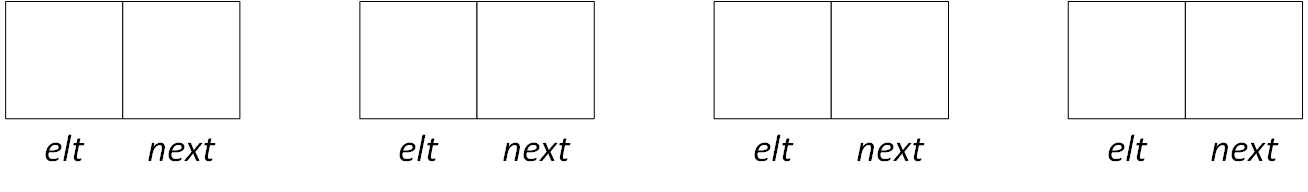
\includegraphics[height=1.85cm]{img/Liste_p_vide_4.png}
%%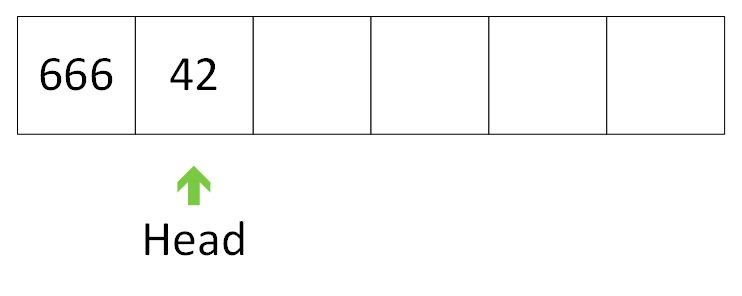
\includegraphics[scale=1,left]{img/2_elts.png}
}
\end{figure}


\texttt{Ajout de 14 en \textit{dernière} position}

\begin{figure}[ht!]
\centering
\centerline{  %%% CENTRAGE HORIZONTAL
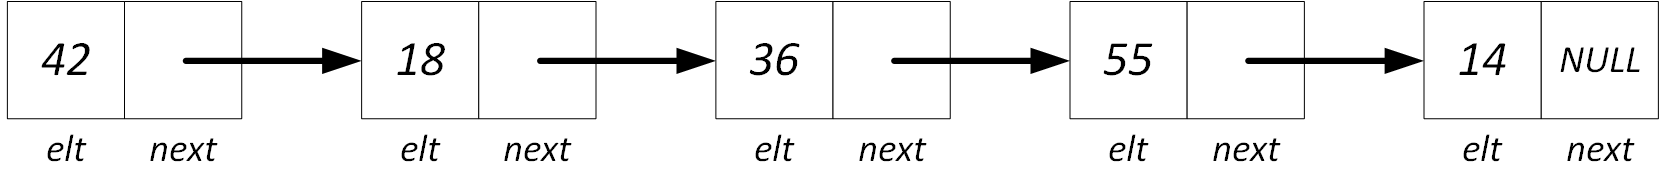
\includegraphics[height=1.85cm]{img/f-2-Liste_p_5.png}
%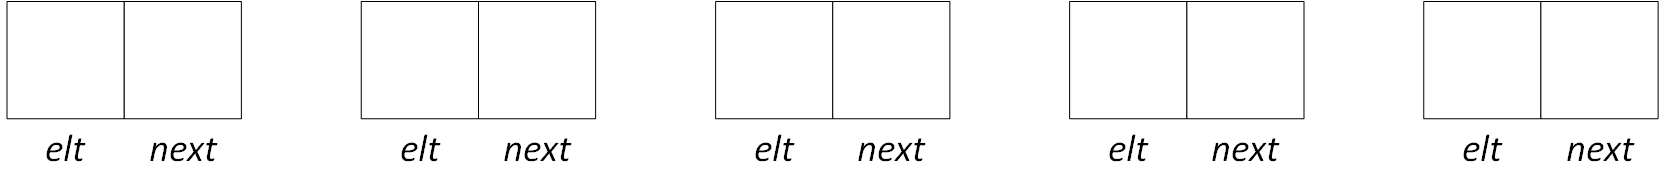
\includegraphics[height=1.85cm]{img/Liste_p_vide_5.png}
%%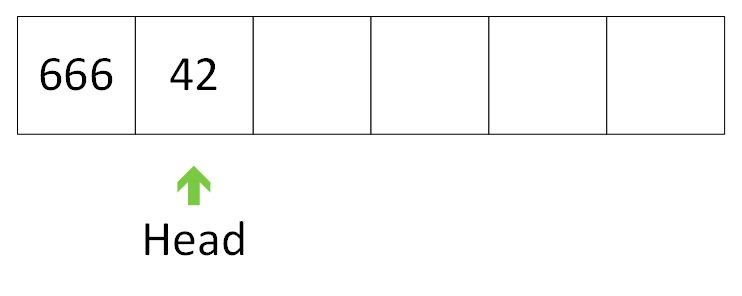
\includegraphics[scale=1,left]{img/2_elts.png}
}
\end{figure}


\texttt{Ajout de 21 en \textit{dernière} position}

\begin{figure}[ht!]
\centering
\centerline{  %%% CENTRAGE HORIZONTAL
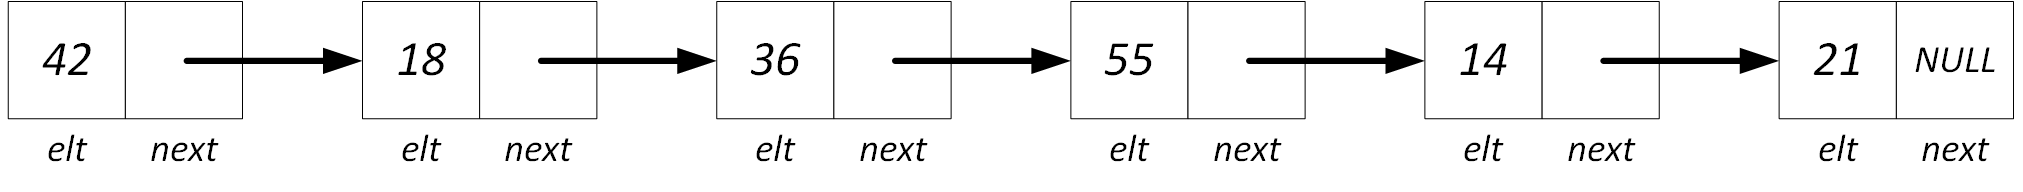
\includegraphics[height=1.85cm]{img/f-3-Liste_p_6.png}
%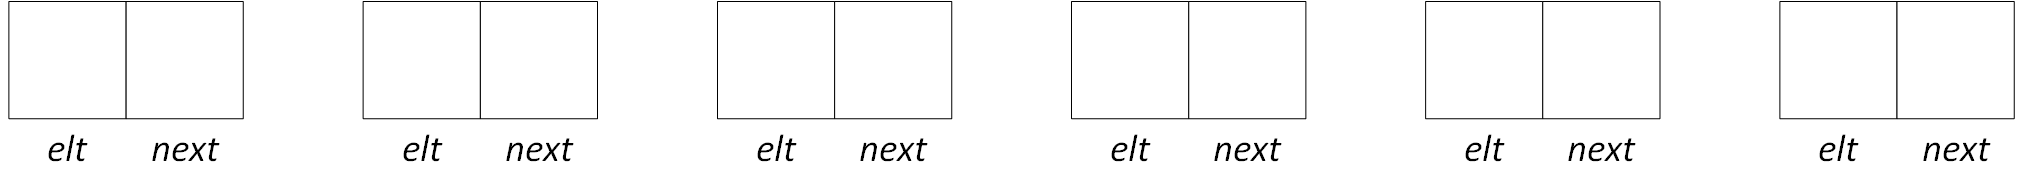
\includegraphics[height=1.85cm]{img/Liste_p_vide_6.png}
%%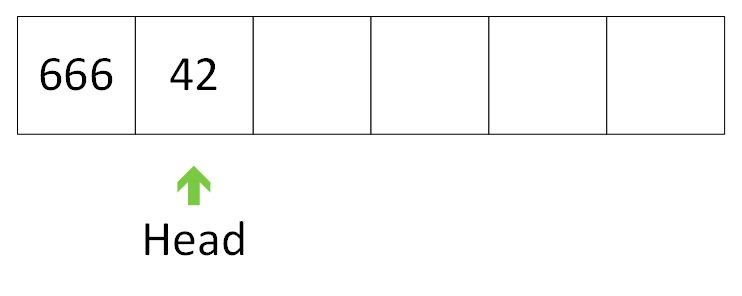
\includegraphics[scale=1,left]{img/2_elts.png}
}
\end{figure}


\texttt{Suppression de la première position}

\begin{figure}[ht!]
\centering
\centerline{  %%% CENTRAGE HORIZONTAL
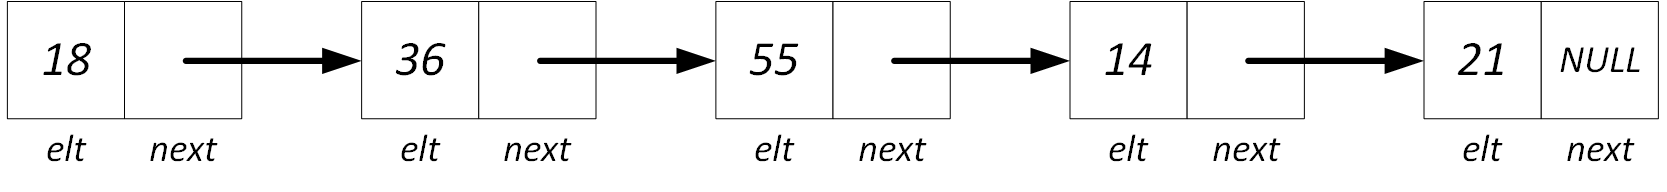
\includegraphics[height=1.85cm]{img/f-4-Liste_p_5.png}
%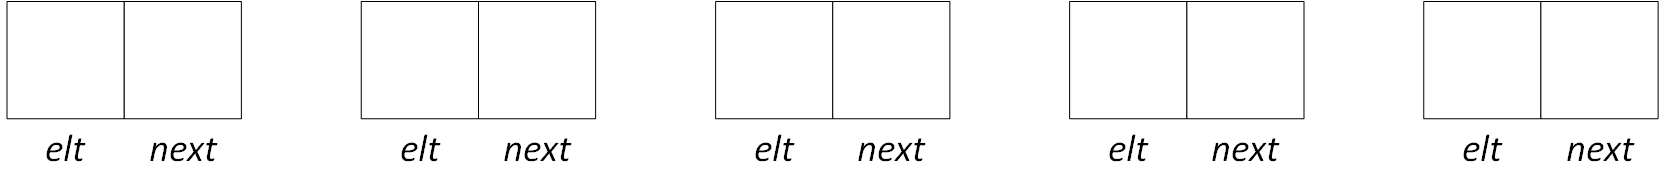
\includegraphics[height=1.85cm]{img/Liste_p_vide_5.png}
%%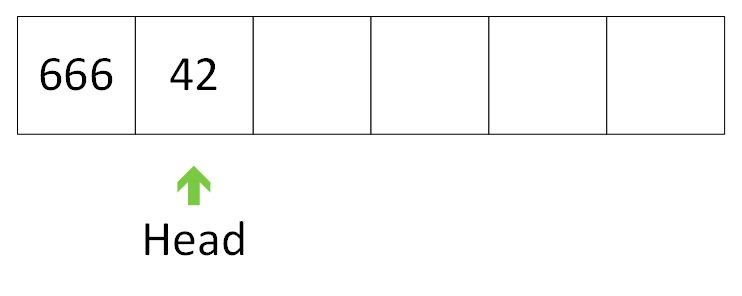
\includegraphics[scale=1,left]{img/2_elts.png}
}
\end{figure}


\texttt{Suppression de la première position}

\begin{figure}[ht!]
\centering
\centerline{  %%% CENTRAGE HORIZONTAL
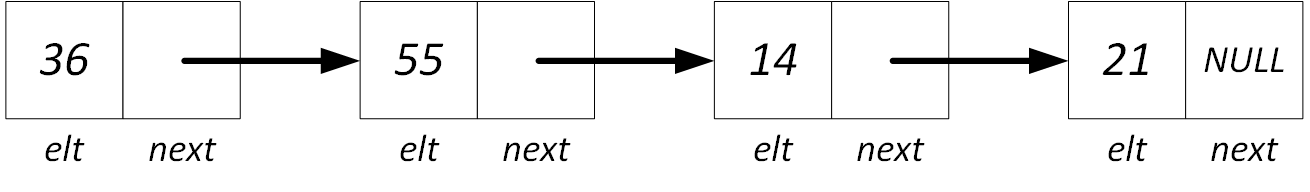
\includegraphics[height=1.85cm]{img/f-5-Liste_p_4.png}
%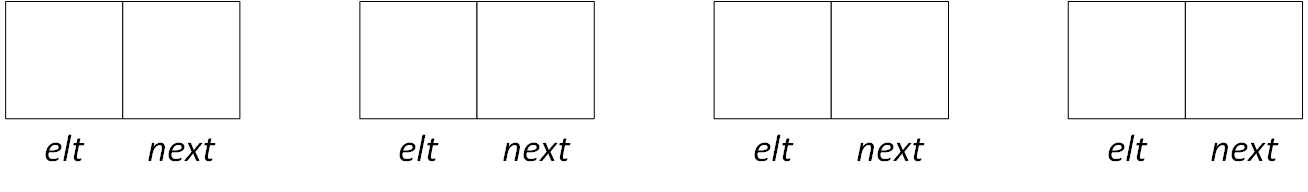
\includegraphics[height=1.85cm]{img/Liste_p_vide_4.png}
%%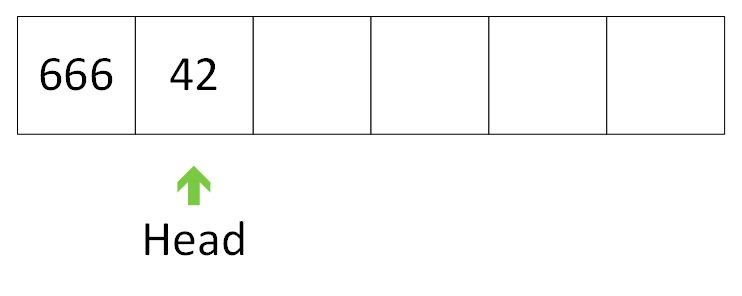
\includegraphics[scale=1,left]{img/2_elts.png}
}
\end{figure}


\texttt{Suppression de la première position}

\begin{figure}[ht!]
\centering
\centerline{  %%% CENTRAGE HORIZONTAL
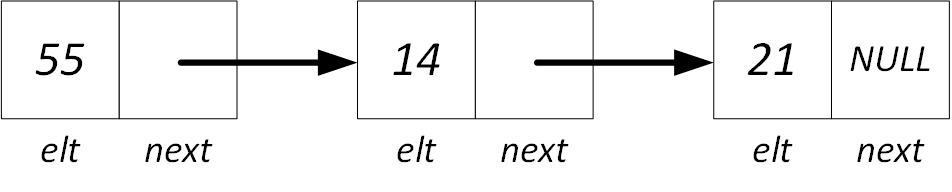
\includegraphics[height=1.85cm]{img/f-6-Liste_p_3.png}
%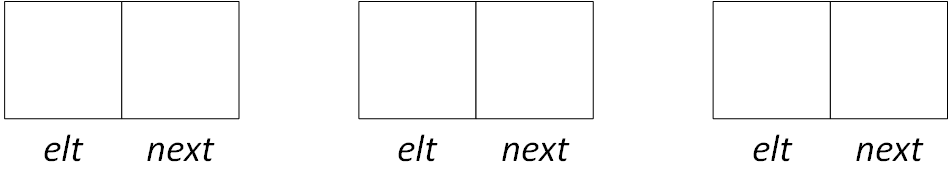
\includegraphics[height=1.85cm]{img/Liste_p_vide_3.png}
%%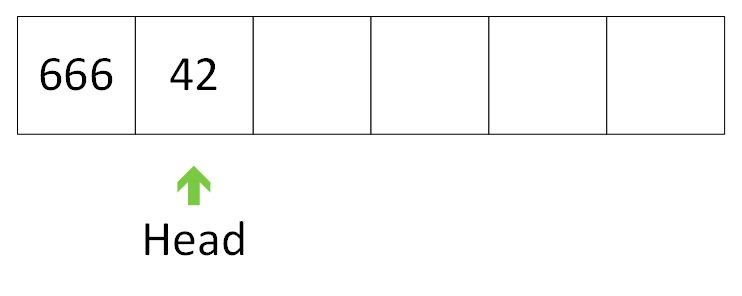
\includegraphics[scale=1,left]{img/2_elts.png}
}
\end{figure}

\bigskip

\end{center}

Structure de données imitée : \textbf{File}

\bigskip



\clearpage

%
\section{Algorithmes (14 points)}

%Dans cet examen, vous allez implémenter avec précisions quelques opérations basiques d'utilisation d'une liste (taille de la liste, récupération du premier élément, récupération du dernier élément, test si la liste est vide, ajout d'un élément à un emplacement précis en poussant les éléments suivants, suppression d'un élément suivi d'une copie des éléments suivants, vider la liste), et vous utiliserez ces opérations pour implémenter une pile et une file.
%
%\smallskip
%
%Le but de l'implémentation est de réutiliser les fonctions que vous écrirez.
%Si vous ne savez pas implémenter une des fonctions, vous pouvez tout de même l'utiliser dans les exercices suivants.

Dans cet exercice, vous allez tout d'abord implémenter avec précisions quelques opérations basiques d'utilisation d'une liste.
Ensuite, vous les réutiliserez pour implémenter une pile et une file.
Si vous ne savez pas implémenter une des fonctions de la partie A, vous pouvez tout de même l'utiliser dans les exercices de la partie B.


%%%%%%%%%%%%%%%%% CENTRAGE
%\vfillFirst

\subsection*{A - Liste à pointeurs (10 points)}

\subsection{(1 point) \'Ecrivez une structure de données \og \textit{my\_list\_p} \fg{} pouvant servir de liste contenant des éléments étant des entiers positifs. Cette liste doit être une liste chaînée utilisant des pointeurs (aucun tableau ne doit être utilisé). }

%\bigskip
\medskip

\begin{center}
\GrilleReponseN{7}
\end{center}

%\bigskip
\medskip

\subsection{(2 points) \'Ecrivez l'implémentation des fonctions suivantes : }

\begin{itemize}
\item \textit{length\_list} : renvoie la taille de la liste, c'est-à-dire le nombre d'éléments contenus
\item \textit{get\_first\_elt} : renvoie le premier élément de la liste
\item \textit{get\_last\_elt} : renvoie le dernier élément de la liste
\item \textit{is\_empty\_list} : renvoie \textit{vrai} si la liste est vide, sinon \textit{faux}
\end{itemize}

%\bigskip
\medskip

\texttt{int length\_list(my\_list\_p *list)}

\begin{center}
\GrilleReponseN{7}
\end{center}

%\medskip

%\vfillLast
%%%%%%%%%%%%%%%%% CENTRAGE

\clearpage

%%%%%%%%%%%%%%%%% CENTRAGE
\vfillFirst

\texttt{int get\_first\_elt(my\_list\_p *list)}

\begin{center}
\GrilleReponseN{7}
\end{center}

\medskip

\texttt{int get\_last\_elt(my\_list\_p *list)}

\begin{center}
\GrilleReponseN{7}
\end{center}

\medskip

\texttt{bool is\_empty\_list(my\_list\_p *list)}

\begin{center}
\GrilleReponseN{7}
\end{center}


\vfillLast
%%%%%%%%%%%%%%%%% CENTRAGE

\newpage

\subsection{(3 points) \'Ecrivez une fonction \og \textit{add\_elt\_at\_pos} \fg{} qui ajoute un élément \textit{elt} à la position \textit{pos} dans la liste \textit{list}. Si la liste est vide, vous créerez la liste et y ajouterez un élément. Si la position est négative, vous renverrez un pointeur \texttt{NULL}. Si la position est supérieure au maximum, l'élément sera ajouté en fin de liste. La position 0 est considérée comme la première position de la liste. }

\bigskip

\texttt{my\_list\_p *add\_elt\_at\_pos(my\_list\_p *list, int elt, int pos)}

\begin{center}
\GrilleReponseN{22}
\end{center}

\newpage

\subsection{(3 points) \'Ecrivez une fonction \og \textit{del\_elt\_at\_pos} \fg{} qui supprime l'élément de la position \textit{pos} dans la liste \textit{list}. Si la liste est vide ou si la position n'existe pas, vous renverrez un pointeur \texttt{NULL}. La position 0 est considérée comme la première position de la liste. (attention aux fuites mémoire) }

\bigskip

\texttt{my\_list\_p *del\_elt\_at\_pos(my\_list\_p *list, int pos)}

\begin{center}
\GrilleReponseN{22}
\end{center}

\newpage

\subsection{(1 point) \'Ecrivez une fonction \og \textit{clear\_list} \fg{} qui vide la liste \textit{list} en supprimant tous les éléments contenus dedans. Vous renverrez un pointeur \texttt{NULL}. }

\bigskip

\texttt{my\_list\_p *clear\_list(my\_list\_p *list)}

\begin{center}
\GrilleReponseN{9}
\end{center}


%\newpage


\subsection*{B - Pile et File avec liste à pointeurs (4 points)}

Vous allez maintenant utiliser les fonctions que vous venez d'écrire pour implémenter des piles et des files.
Vous devez réutiliser les fonctions existantes (non pas en les réécrivant, mais en les appelant).
N'hésitez pas à relire vos réponses de la partie \textit{Questions} pour vous aider.

\subsection{(1 point) \'Ecrivez une fonction \og \textit{push} \fg{} pouvant servir à empiler un élément dans une liste. }

\bigskip

\begin{center}
\GrilleReponseN{9}
\end{center}

\newpage

\subsection{(1 point) \'Ecrivez une fonction \og \textit{pop} \fg{} pouvant servir à dépiler un élément depuis une liste. }

\bigskip

\begin{center}
\GrilleReponseN{10}
\end{center}

\bigskip



%\newpage

\subsection{(1 point) \'Ecrivez une fonction \og \textit{enqueue} \fg{} pouvant servir à enfiler un élément dans une liste. }

\bigskip

\begin{center}
\GrilleReponseN{10}
\end{center}

%\newpage

\subsection{(1 point) \'Ecrivez une fonction \og \textit{dequeue} \fg{} pouvant servir à défiler un élément depuis une liste. }

\bigskip

\begin{center}
\GrilleReponseN{10}
\end{center}

\bigskip

\end{document}
